%%%%%%%%%%%%%%%%%%%%%%%%%%%%%%%%%%%%%%%%%%%%%%%%%%%%%%%%%%%%%%%%%%%%%%%%%%%%%%%%%%%%%%%%%
% SECTION HYDRODYNAMIC SIMULATIONS 
%%%%%%%%%%%%%%%%%%%%%%%%%%%%%%%%%%%%%%%%%%%%%%%%%%%%%%%%%%%%%%%%%%%%%%%%%%%%%%%%%%%%%%%%%

\chapter{Hydrodynamic Simulations}
\section{2D Simulations}
The physics of 2D hydrodynamics is qualitatively very similar but quantitatively very different to the 3D case. Concepts such as hydrostatic equilibrium or the Schwarzschild criterion can be applied in 2D as well as in 3D, but the resulting flows will have different properties. Turbulence for instance in the 2D case transfers kinetic energy from smaller eddies to larger eddies, while in the 3D case the opposite happens (for an introduction in the subject see \citet{boffetta}). We expect hence the entrainment mass ratio to be different between the 2D and 3D cases. 

Nevertheless, since 2D simulations are computationally so cheap, they are a very useful tool to familiarize with the code and to run tests in order to setup bigger and more expensive 3D runs. In our case we needed a rough estimate of the entrainment rate, of the boundary migration velocity and of the convective turnover timescale. Specifically, it is necessary to make sure that convection reaches a stable regime over a fairly large time domain (in our case at least $5$ convective turnover times), to correctly collect the data that characterizes the boundaries.
	
\subsection{Simulations setup}
The physical setup used for our simulations is the so called "box in a star" method, meaning that we simulate some relatively very small internal region of a star. 

In our case for the 2D runs it will be a box of $2.50 \times 10^{9} \ \mathrm{cm}$ on the $x$ axis and $1.25 \times 10^{9} \ \mathrm{cm}$ on the $y$ axis. Gravity is constantly pointing downward on the $y$ axis with a magnitude of $10^3 \ \mathrm{cm/s^2}$. This generates a pressure stratification in the fluid that covers approximately three pressure scale heights. 

The controlling parameter to initialize the fluid stratification is the temperature gradient. In our case we divided the simulated region in three parts. The bottom region (labeled as $1$) starts at the lower boundary and reaches $1/3$ of the domain, the central (labeled as $2$) proceeds until the middle, and the upper one (labeled as $3$) reaches the upper boundary, as shown in Figure (\ref{fig:twin}). Convection will be generated in the central region. We chose to initialize a larger stable layer above rather than a symmetric setup because, as the first tests showed, the upper boundary is always softer and hence entrains more material. This is in agreement with what found by \citet{meakin}. We define a parameter $\alpha_{i}$ ($i=1, 2, 3$) which is nothing but the fraction of the $\nabla$ over the $\nabla_{\mathrm{ad}}$. As seen in previous sections $\alpha_{i}<1$ implies stability in the region $i$, instability otherwise. 

We always initialized the setup with $\alpha_{1} = \alpha_{3}$ much smaller than $1$; and $\alpha_{2}=0.99$, which means a very precarious situation in terms of stability in the second region. 

A heating function furthermore heats the second region with a gaussian profile (see Figure \ref{fig:twin}) to stimulate convection. Without it the system would never become convective in the first place, since hydrostatic equilibrium is fulfilled everywhere. Furthermore the heating function keeps the system convectively unstable over time. In fact without the constant energy generation because of heat mixing and numerical viscosity, the system would soon reach again a stable configuration of hydrostatic equilibrium. The heating mimics the energy generation in deep stellar interiors due to nuclear burning. The choice of a Gaussian profile is a common practice in stellar physics. On the one hand we require that the heating is peaked deep inside the convective region and that it does not influence the stable layers, on the other hand it is preferable not to use functions with discontinuity, because this might generate shock waves that propagate into the system.

The values of $\alpha_{1}$ and $\alpha_{3}$ are controlling parameters for the bulk-Richardson number, since they are proportional to $\Delta b$. The advantage of simulating a strip of convection between two stable layers (miming a Shell convection) instead of a convective region at the bottom that grows upward (core convection-like) is twofold. It gives us two convective boundaries to study per run instead of one, and we avoid to insert a wall boundary (see next paragraphs) in contact with convective motions, which is a very unphysical setup. 

One of the hardest tasks has been to generate the correct amount of heating such that the turbulence standard deviation \textit{at the interface} was constant during the run (which is one of the ingredients of the bulk-Richardson number, hence one of the parameters we want to control in order to perform a differential study). In order to do that, the heating rate decreases over time in an hyperbolic fashion such that, at $t=10^5 \ \mathrm{s}$, the total heat generation is reduced to $50 \%$ of the original amount.

\begin{figure}[t]
\centering
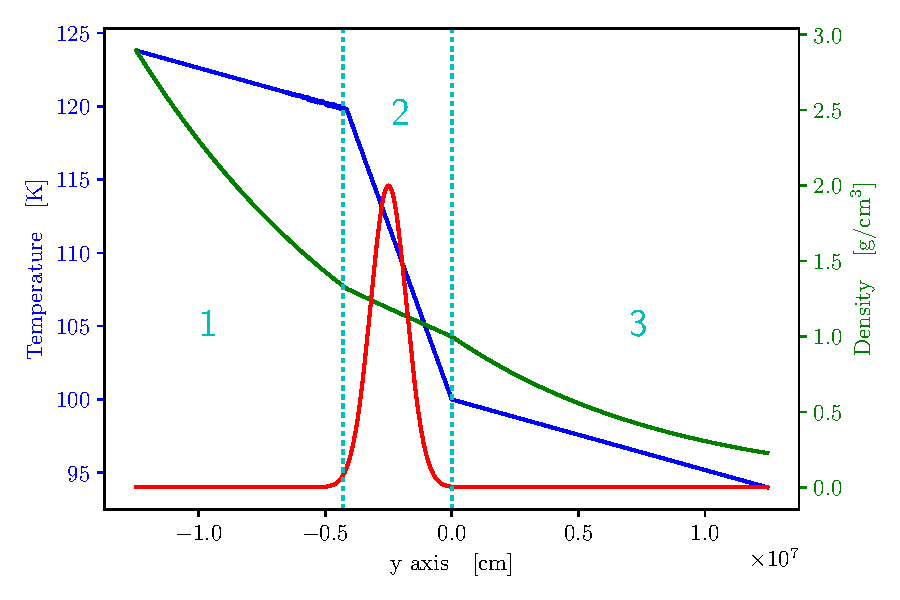
\includegraphics[width=10cm]{./img/twin.pdf}
\caption{Example of initial temperature (blue) and pressure (green) profile along the $y$-axis. The red curve represents the shape of the heating function in arbitrary unit. Notice the little perturbations in temperature between the first and second region (see text).}
\label{fig:twin}
\centering
\end{figure}
At the bottom of the convective region small perturbations in temperature and Mach number had been imprinted on the stratification in order to break the initial symmetry of the system.

A wide range of boundary conditions have been tested for this problem. For the vertical direction we used wall boundaries. As previously stated, in our first setup we used to stimulate convection at the bottom of the simulated region, but implementing periodic boundaries in the horizontal direction (that definitely provide the most physical situation) a shear flow appeared in both the stable and convective region at the onset of convection. We then tested reflective boundaries and wall boundaries. In the first case we observed a mass loss (very likely because of a bug in the code). In the second case after a few tens of minutes of the onset of convection, a spike in the Mach number at the boundary appeared, and the code crashed. Interestingly enough, the spike appeared always at the left boundary. For this reason we initially suspected another bug in the code. What actually used to happen is that some fluid stagnated right above the convective boundary (specifically the first column of cells on the left) and over time a massive temperature gradient was established. We suppose that this computational artifact appeared only on one side of the grid because the iterative linear solvers implemented in SLH are not perfectly symmetric. This is generally not a source of problems unless in specific pathologic cases as the one we had to face. We then tested a new setup, where convection was stimulated in the central region of the domain. By implementing periodic boundaries the same shear flow appeared, but only after a few tens of hours of simulated time, which allowed us to collect enough data for the analysis. As we will explain this is not a perfectly physical solution, since internal modes can bounce on them and be reflected.


As briefly explained in the previous sections, we initialized two different passive scalars inside the regions one and three. Recall that passive scalars are just like dyes in the fluid which in no way influence the dynamics of the system, nor do they diffuse. The passive scalar one and three (initialized in the regions 1 and 3) will be used to compute the entrained mass, i.\ e.\ for every time step we integrate the passive scalar densities in the convective region and obtain the total entrained mass at each boundary. The two passive scalars are also used in order to define the boundary topology (i.\ e.\  position and width), by looking at the biggest drop in passive scalar density.

As previously stated our goal is to perform a \textit{differential} study of the bulk-Richardson number and the CBM problem. This implies running simulations with different values of $\Delta b$ and $\sigma_{\mathrm{T}}$ at different resolutions. Because 2D simulations are computationally so cheap, we managed to run a  sufficient amount of them in a short time. With the code 2d0.10-100 we will refer to a 2-dimensional run with $\alpha_{1} = \alpha_{3}=0.1$ and $100 \%$ of the heating referring to the fiducial value of $3.6 \times 10^{15} \, \mathrm{erg/s}$.

We run in 2D on a $2048 \times 1024$ uniform Cartesian grid. It is worth remarking that when doing CFD with a higher resolution, one not only better resolves the features of the system, but also decreases the numerical viscosity (increases the Reynolds number). This is the reason why we chose this grid setup: we want to keep cells squared and keep viscosity a scalar quantity, and prevent it from becoming a tensorial one. In the next section we will perform a convergence study, in order to understand which roles the resolution and the viscosity play in the phenomenon of convective entrainment.

We performed the runs on our local cluster at HITS. Every job required about $4.5 \times 10^{4}$ cpu hours on bridge architecture, and roughly the half of it on Haswell architecture. We saved one output file every $100$ time steps, in order to both save memory and to avoid wasting too much computing time in I/O processing.


\subsection{Evolution of a 2D run}\label{single2d}

Let us consider the setup 2d0.1-100. 

Convection starts at $t \simeq 150 \, \mathrm{min}$. Because of the already mentioned implicit time stepping, the lower the Mach number, the bigger the time step, allowing us to save a huge amount of computational resources before the rise of convection. A remarkable difference in computational efficiency compared to an explicit time stepping was also observed during the convective regime, as long as the Mach number was below $10 \%$, which has always been our case.

\begin{figure}[t!]
      \centering
      \subfloat[Mach number profile over time.]{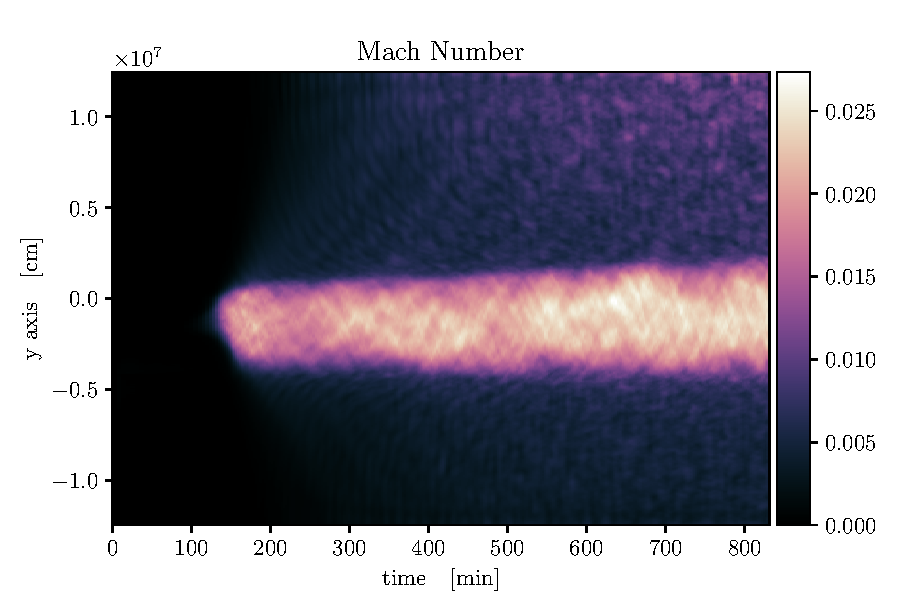
\includegraphics[width=12cm]{./img/mach.pdf}\label{fig:2dmachprofile}}
     \centering
	\hfill
	\subfloat[Entrainment of the third passive scalar from the upper stable region (region 3) in the convective region.]{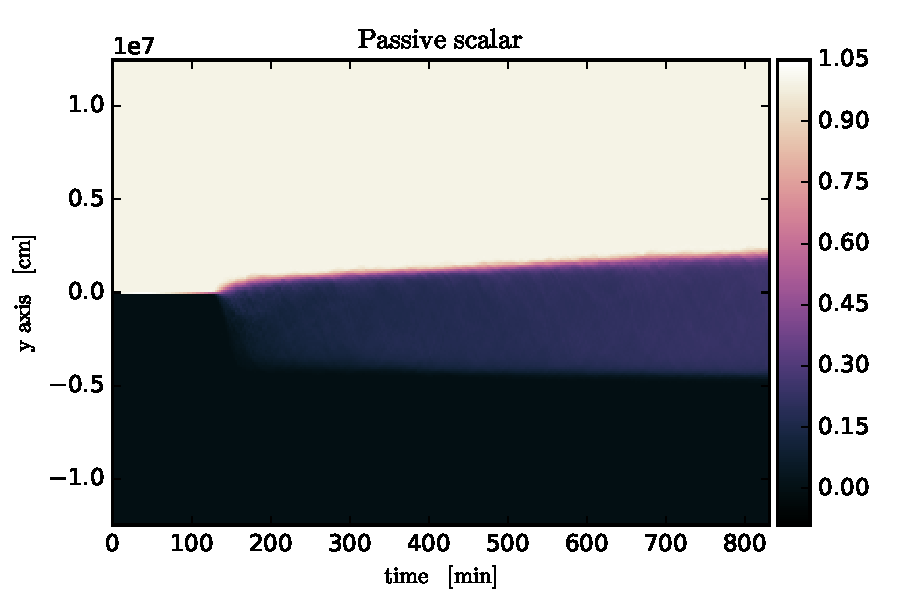
\includegraphics[width=12cm]{./img/ps2.pdf}\label{fig:2dpsprofile}}
	\caption{Time evolution of a 2D run for the Mach number and the third passive scalar (average on the horizontal direction).}
	\label{fig:2dsinglefirst}
\end{figure}
In Figure \ref{fig:2dmachprofile} we plot the profile of the Mach number over the simulated time. Convection starts at around $t=150 \mathrm{min}$ in the central region (region 2), while the upper and lower region remain stable. Some time is needed for convection to develop, because the fluid needs to be heated to an unstable configuration. One can also observe that the convective region expands over time, i.\ e.\ the upper boundary moves upward and the lower boundary downward. Two remarks need to be made. 

\begin{figure}[t!]
\centering
\subfloat[Advection of the upper passive scalar (from region 3) at the onset of convective motions, at $t \simeq 150 \ \mathrm{min}$.]{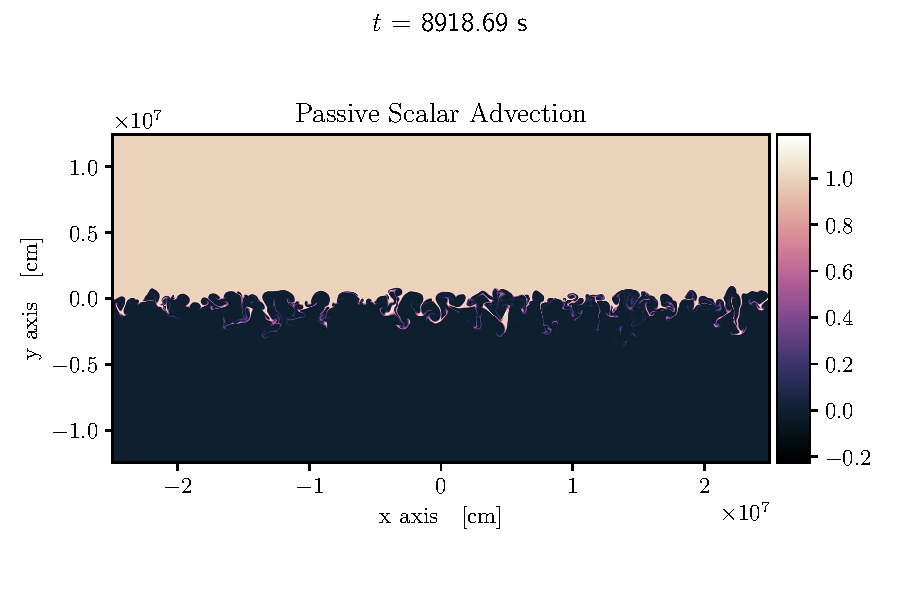
\includegraphics[width=12cm]{./img/passive2acc1.pdf}\label{fig:passiveacc1}}
\hfill
\subfloat[The same passive scalar of above, advected at $t \simeq 800 \ \mathrm{min}$. This defines the topology of the boundary.]{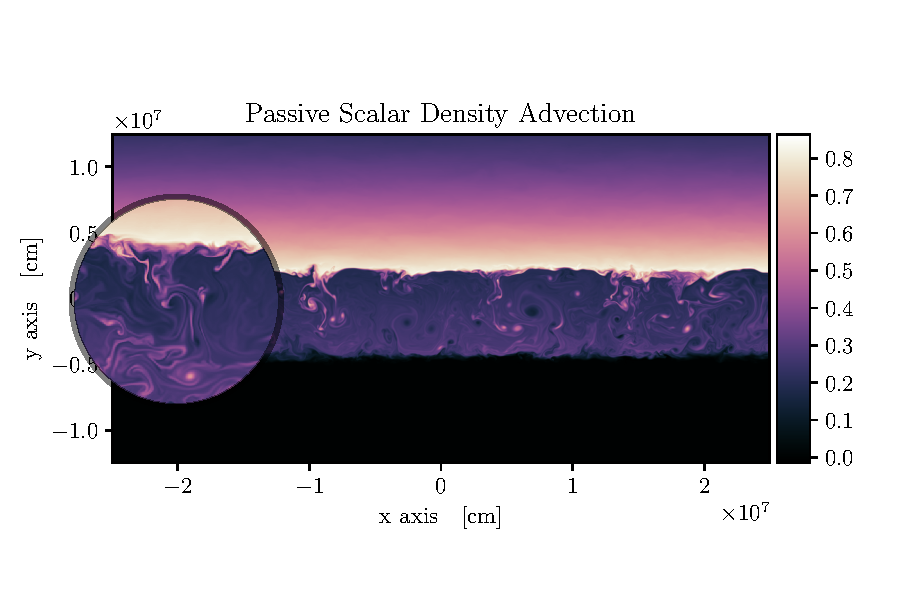
\includegraphics[width=12cm]{./img/passive2acc2.pdf}\label{fig:passiveacc2}}
\caption{Advection of the passive scalar initialized in the central region over the simulated time}
\label{fig:2dpassive}
\end{figure}

First of all the Mach number is stable over time, thanks to the heating function that we implemented, featuring a decrease of heat generation as previously explained. 
Second it is clear that some internal modes are excited by the convective blobs when they hit the stable layers and they propagate through them. They appear more significant in the upper region and to a certain extent this is true, but mainly this is due to the fact that the speed of sound there is lower. The difference is not so dramatic when plotting the absolute velocity. Two interesting questions remain without answer. First of all it is impossible to tell to which extent the dynamic of the boundary is influenced by these modes. Second of all it is possible that the chemical mixing due to these modes in the stable stratification might have a significant impact on the evolution of a star, which is obviously not considered in 1D simulations. We believe that further investigations of this hypothesis are needed.

In Figure \ref{fig:2dpsprofile} we plot the upper passive scalar (initialized in the region 3), which over time is entrained by convection. We clearly see the motion of the boundaries that over the $800 \ \mathrm{min}$ of simulated time move gradually (and roughly linearly in time) upward and downward. As previously mentioned the first passive scalar was initialized in the lower region (region 1), and consequently advected into the convective region. A Lagrangian study of entrainment consists in quantifying the amount of passive scalar ingested at each boundary over time, i.\ e.\ integrating each passive scalar density over the convective region at every time step, and analyze the growth of this quantity over time.

As previously mentioned the two passive scalars are also used to define the boundary topology, position, and width. In Figure (\ref{fig:passiveacc1}) we show the upper passive scalar at the onset of convection. The rise of the first convective blobs is clearly visible. In the next $650 \mathrm{min}$ part of this dye will be entrained from the upper stable layer in the convective region as it can be clearly seen in Figure (\ref{fig:passiveacc2}). We define the boundary position as the surface where the gradient of the concentration of the upper passive scalar changes the most. This holds for both the upper and lower boundary.
  
For the runs with lower resolution this method worked perfectly, but when moving to a higher resolution a problem appeared.  In Figure (\ref{fig:topology})  in the middle of the convective layer some blobs of entrained material are visible, that even when fully in a convective regime still contain a very high passive scalar density. This is due to the fact that the higher the resolution, the lower the numerical diffusion.
  
\begin{figure}[t!]
\centering
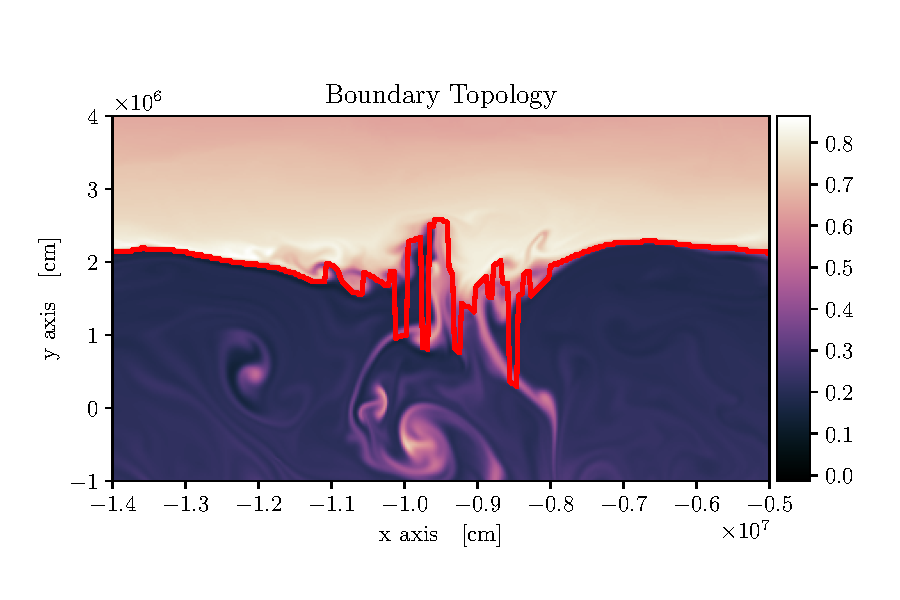
\includegraphics[width=10cm]{./img/topology.pdf}
\caption{The detected upper boundary topology over the passive scalar density (see text).}
\label{fig:topology}
\centering
\end{figure}

\begin{figure}[b!]
\centering
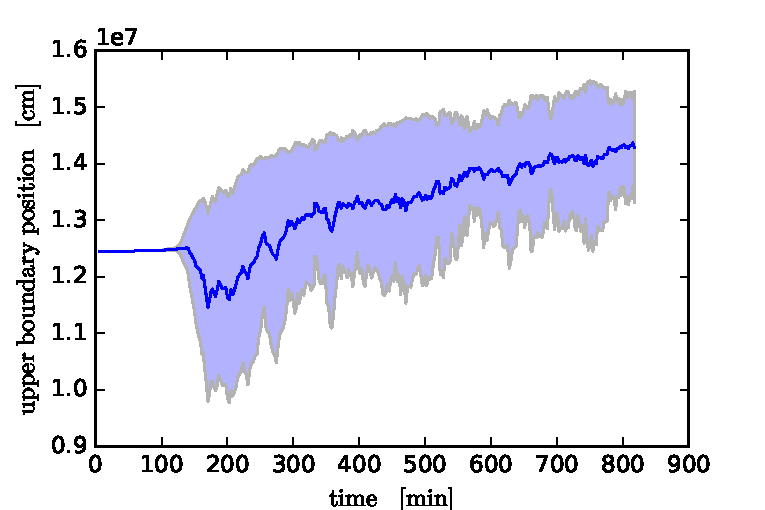
\includegraphics[width=0.7\textwidth]{./img/boundpos.pdf}
\caption{Boundaries positions over time. Shaded regions represent the boundary thickness (see text). Blue lines represent the upper boundary, green lines the lower boundary.}
\label{fig:boundpos}
\end{figure}
As a result, the topology is characterized by multiple analytical discontinuities. This suggests that our prescription is only able to provide mean values for the boundary position and width, and not local values. Hence these discontinuities should not be necessarily interpreted as a failure of our method, rather as phenomenon which encapsulates the more turbulent and stochastic regime that we approach by enhancing the resolution, that consequentially can only be treated from a statistical standpoint.

For the 3D runs this problem does not appear, because of the different turbulent structure of convection. In fact in the 3D case, turbulent blobs decay in smaller and smaller blobs (contrarily to what happens in the 2D case), and this natural process helps brake down these spikes (at least at the resolutions we performed out runs).


\begin{figure}[t!]
  \centering
    \subfloat[Buoyancy jump over time.]{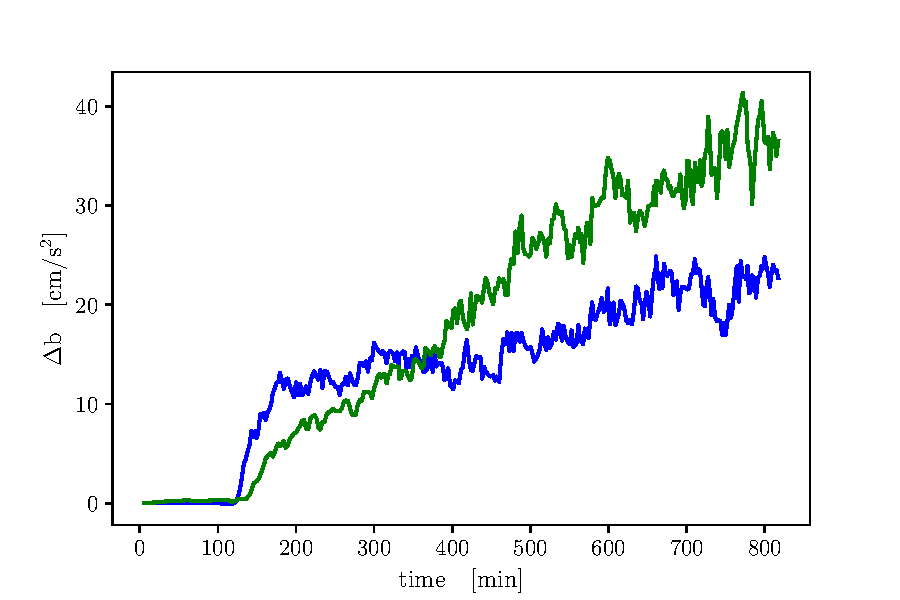
\includegraphics[width=0.5\textwidth]{./img/delb.pdf}\label{fig:delb}}
      \hfill
        \subfloat[Turbulence length scale over time.]{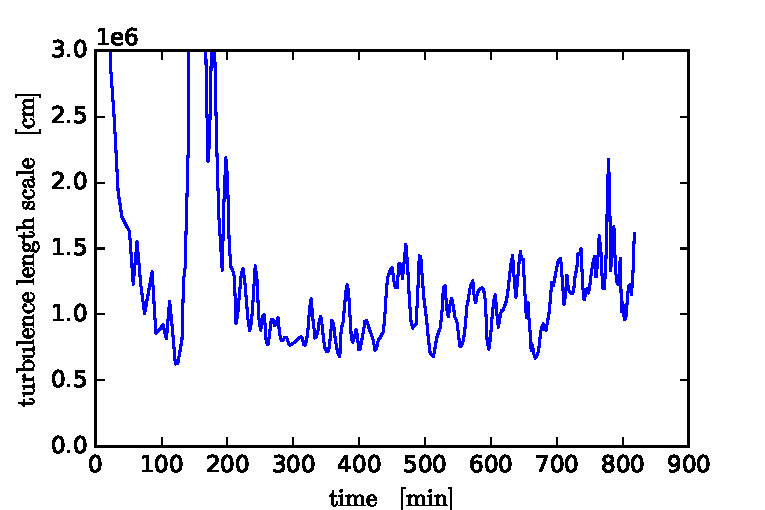
\includegraphics[width=0.5\textwidth]{./img/len.pdf}\label{fig:len}}
	\hfill
  \centering
    \subfloat[Turbulence standard deviation over time.]{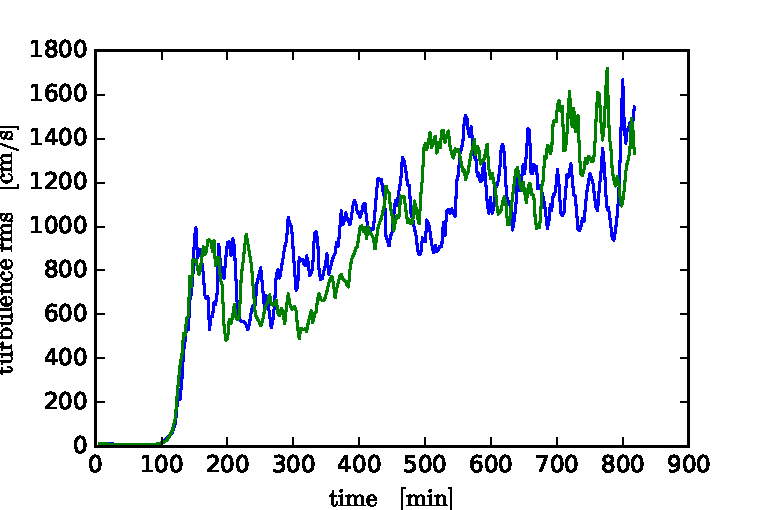
\includegraphics[width=0.5\textwidth]{./img/sigt.pdf}\label{fig:sigt}}
      \hfill
        \subfloat[Entrained mass over time.]{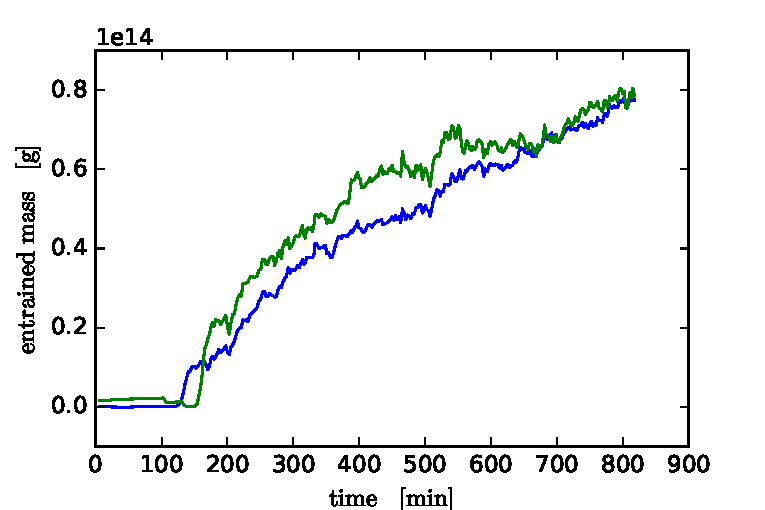
\includegraphics[width=0.5\textwidth]{./img/ent.pdf}\label{fig:ent}}
	\caption{Time evolution of the parameters needed to compute the bulk-Richardson number and of the entrained mass at the boundaries. Blue lines represent the upper boundary, green lines the lower boundary.}
	\label{fig:2dparam}
\end{figure}
We plot in Figure (\ref{fig:boundpos}) the boundaries positions over time. Shaded regions represent the boundary thickness (calculated as the boundary position standard deviation). Convection clearly starts at about $t=150 \, \mathrm{min}$. After a transition period of about $50 \mathrm{min}$ we can clearly see that there is a migration of the upper boundary upward and of the lower boundary downward, which is fairly stable over the run. Specifically, in the upper case it starts in the middle of the simulated region and ends up at $\simeq 2.0 \times 10^{6} \ \mathrm{cm}$, for the lower case it starts at $\simeq - 3.1 \times 10^{6} \ \mathrm{cm}$ and moves downwards to $\simeq - 4.5 \times 10^{6} \ \mathrm{cm}$. The boundaries thickness is also overall stable. As previously mentioned an Eulerian study is impracticable for this phenomenon, because it is hard to quantify how much of the boundary migration in an Eulerian frame is due to the entrainment and how much due to the adiabatic expansion of the fluid. We observe a decrease in density in the central region of a few percent, and we presume the volume expands consequently. 

In Figure (\ref{fig:2dparam}) we plot the parameters relevant to our analysis. 
The first ingredient of the bulk-Richardson number is the buoyancy jump $\Delta b$, that we plot in figure \ref{fig:delb}. In both cases there is an increasing trend, more significant in the lower boundary. This plot shows one of the biggest challenges of running simulations to study differentially the bulk-Richardson number: it is extremely hard to obtain a run where all the parameters ($\Delta b$, $L$, $\sigma_{\mathrm{T}}$ and $M_{\mathrm{E}}$) are constant over time. Hence one finds itself in the inconvenient situation of having to average over values that span a full order of magnitude with a strong increasing or decreasing trend, and the quality of the analysis is consequentially affected by this uncertainty. 

Notice that the lower boundary is stiffer than the upper one (the buoyancy jump is higher, hence the bulk-Richardson number) even if in the initial setup the Brunt-Väisälä frequency is the same for the two stable regions. Recall that the Brunt-Väisälä frequency $N^2$ is the quantity we integrate in equation (\ref{eq:buoyancyjump}) over the boundary thickness in order to calculate $\Delta b$. Looking at Figure (\ref{fig:brunt}) it is clear that at the convective boundaries spikes arise during the simulation in the Brunt-Väisälä frequency, and in the lower case it is more pronounced. Obviously when integrated over the interface, this gives rise to a bigger buoyancy jump. These spikes in the Brunt-Väisälä frequency at the interfaces were also found by \citet{viallet2013}, \citet{arnett2015}, \citet{cristini}.

\begin{figure}[t!]
\centering
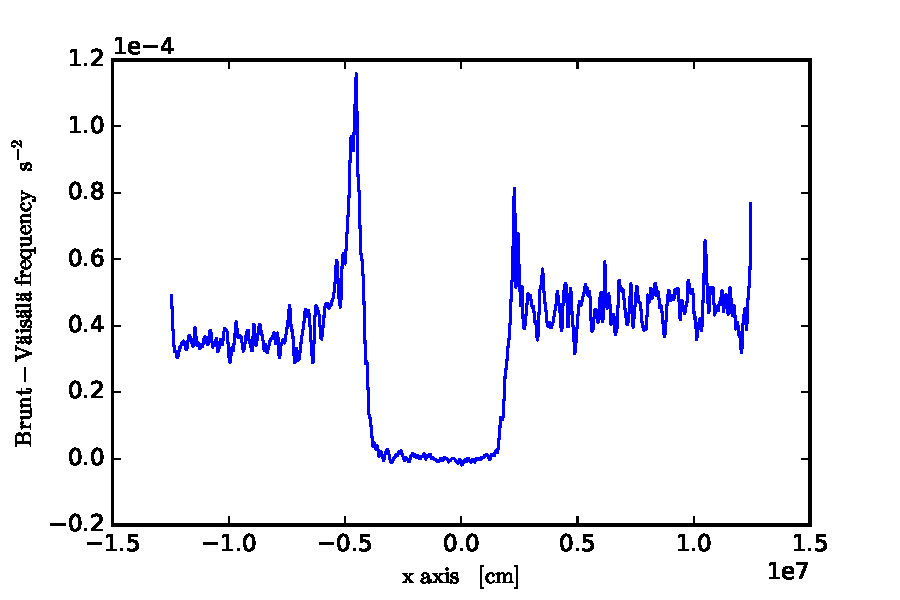
\includegraphics[width=0.7\textwidth]{./img/brunt}
\caption{Horizontal average of the Brunt-Väisälä frequency at about $t=500 \ \mathrm{min}$.}
\label{fig:brunt}
\end{figure}
In Figure (\ref{fig:len}) we plot the turbulent length scale $L$ over time. In this case we only calculated $L$ at the center of the convective layer, so this value will be used both for the upper and lower boundary analysis. The length scale at the interfaces has a value which is overall comparable, but it is affected by some spikes, reason for which we decided to calculate it in a fully convective region. The turbulent length scale is the parameter that takes more time to stabilize, becoming ultimately stable at around $t = 300 \, \mathrm{min}$. 
 
\begin{table}[b!]\caption{Boundaries parameters for the 2d0.10-100 run, U stands for the upper boundary, L for the lower boundary. The errors are the standard deviations on the mean value.}
 \begin{tabular}{lccccc}
	 \toprule
	 Run &$\Delta b  $&$\sigma_{\mathrm{T}}$ & $L$&$Ri_{\mathrm{B}}$&$\dot{M}_{\mathrm{E}}$ \\
		    & $(\mathrm{cm \, s^{-2}})$&$(\mathrm{cm \, s^{-1}})$&$(10^5 \, \mathrm{cm})$ & & $(10^9 \, \mathrm{g \, s^{-1}})$ \\
	  	\midrule
		2d0.7-0.01U&$ 18.17 \pm 3.62 $&$1118 \pm 202 $ &  $10.88 \pm 2.56 $ & $17.07 \pm 7.41 $ & $1.287 \pm 0.006$\\
		2d0.7-0.01L &$27.68 \pm 7.18$&$1190 \pm 218$ & $10.88 \pm 2.56$ &  $21.62 \pm 6.54$ & $0.913 \pm 0.002$\\
		\bottomrule
	\end{tabular}\label{2dsingletab}
 \end{table}
In Figure (\ref{fig:sigt}) we plot the standard deviation of the turbulence absolute Mach number at the convective interfaces over time. It is overall constant, with a slight trend to increase. This result has been obtained after extensive tests to correctly tune the heating function. It is in fact extremely hard to forecast the turbulence velocity by the heating generation and its time evolution. This problem perfectly shows the non-linearity of hydrodynamics as a theory.

In Figure (\ref{fig:ent}) the entrained mass over time. As already mentioned we will perform a Lagrangian study of entrainment, because it is impracticable to quantify how much of the boundary migration is due to the entrained mass or to the adiabatic expansion of the fluid. After an initial spike of entrained mass, we notice that also the entrainment rate stabilizes. We calculate the entrainment rate by fitting the entrained mass over time between $t = 300 \, \mathrm{min}$ until the end of the simulation, and by taking the angular coefficient of the resulting fit. 

\begin{figure}[t!]
\centering
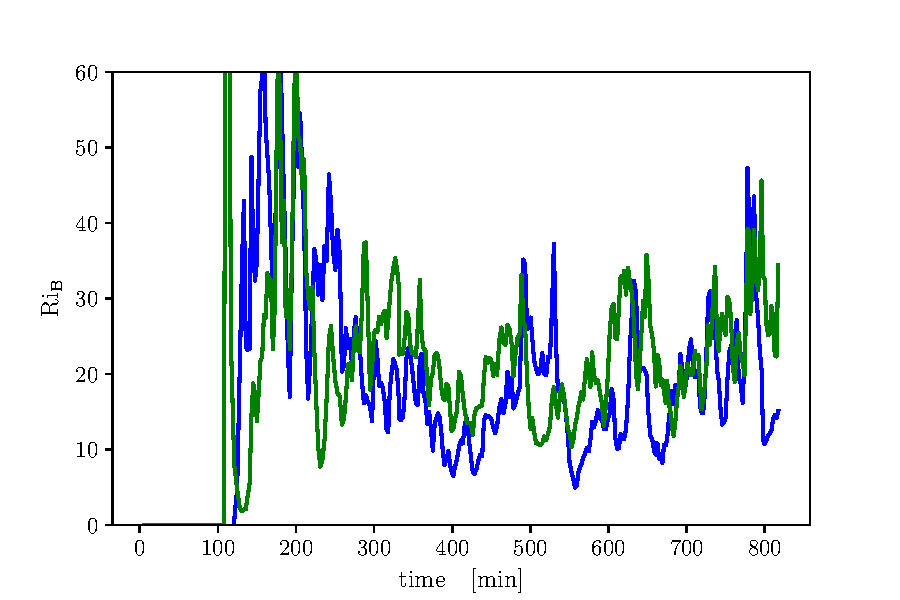
\includegraphics[width=0.7\textwidth]{./img/bulk.pdf}
\caption{Time evolution of the bulk-Richardson number. The blue line represents the upper boundary, the green line the lower one.}
\label{fig:bulk}
\centering
\end{figure}
We show in Figure (\ref{fig:bulk}) the bulk-Richardson number over time. Blue lines represent the upper boundary, green lines the lower boundary. At around $t=\mathrm{300 \, min}$, when the entrainment becomes linear and we start our analysis, the bulk-Richardson number still oscillates over half an order of magnitude. This obviously deeply affects our data analysis, making necessary a large amount of runs to collect as much data as possible. This also makes a differential study of the entrainment over time impracticable. 

For every 2D or 3D run we will collect the relevant parameters and present them in the layout of Table (\ref{2dsingletab}).

\subsection{Resolution study}

\begin{figure}[t!]
  \centering
  \subfloat[Mach number profile for the $2048 \times 1024$ run.]{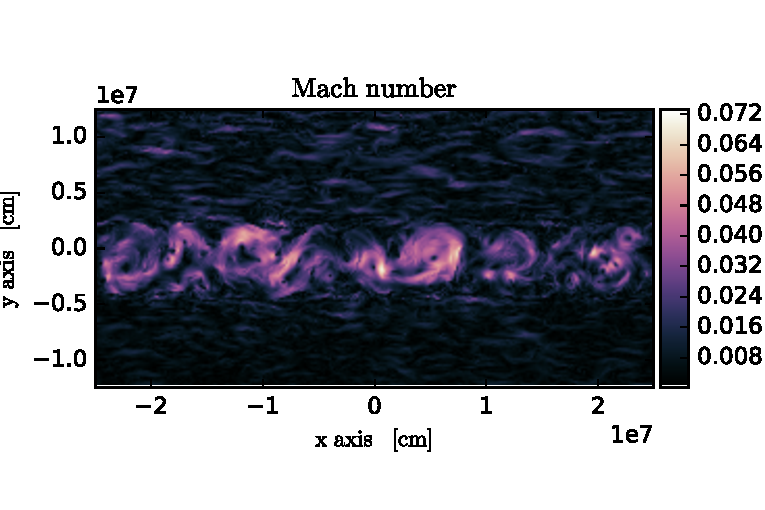
\includegraphics[width=12.cm]{./img/machhighres.pdf}\label{fig:machhighres}}
  \centering
      \hfill
    \subfloat[Mach number profile for the $512 \times 256$ run.]{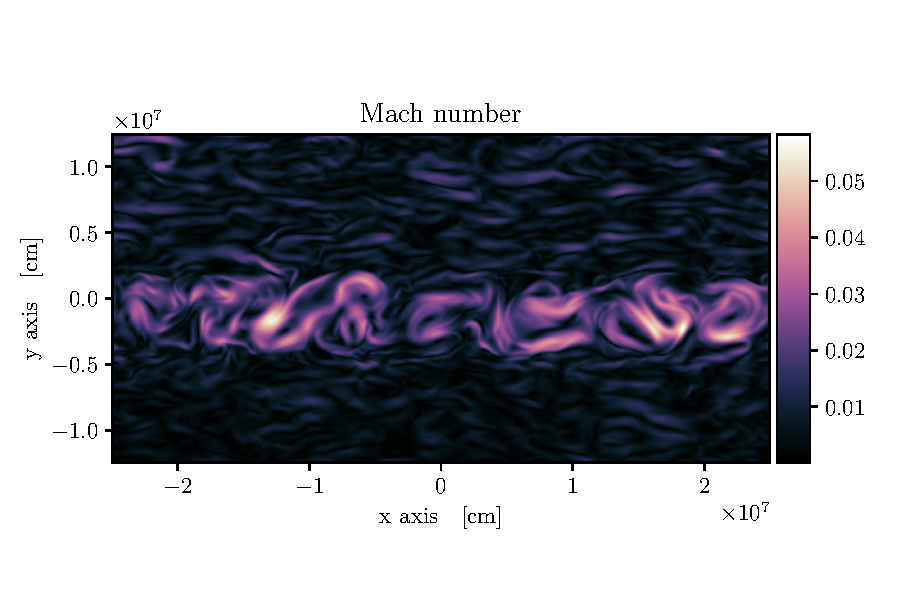
\includegraphics[width=12.cm]{./img/machlowres.pdf}}
    \caption{Turbulent structures at different resolutions at about $t=500 \ \mathrm{min}$. Notice the higher Mach number in the $2048 \times 1024$ run due to lower numerical viscosity (see text).}
    \label{fig:differentialmach}
 \end{figure}

\begin{table}[t!]\caption{Boundaries parameters for the high, medium, and low resolution runs.}
 \begin{tabular}{lccccc}
	 \toprule
	 Run &$\Delta b  $&$\sigma_{\mathrm{T}}$ & $L$&$Ri_{\mathrm{B}}$&$\dot{M}_{\mathrm{E}}$ \\
		    & $(\mathrm{cm \, s^{-2}})$&$(\mathrm{cm \, s^{-1}})$&$(10^5 \, \mathrm{cm})$ & & $(10^9 \, \mathrm{g \, s^{-1}})$ \\
	  	\midrule
		$2048 \times 1024$ U&$ 18.17 \pm 7.41  $&$1118 \pm 202 $ &  $10.88 \pm 2.56 $ & $17.07 \pm 7.41 $ & $1.287 \pm 0.006$\\
		$1024  \times 512$ U &$15.48 \pm 2.31$&$1020 \pm 196$ & $11.07 \pm 3.30$ &  $17.69 \pm 8.40 $ & $1.255 \pm 0.013$\\
		$512 \times 256$ U &$12.82 \pm 2.40$&$970 \pm 233$ & $11.50 \pm 1.71$ &  $17.60 \pm 7.66$ & $1.174 \pm 0.016$\\
		$2048 \times 1024$ L&$ 27.62 \pm 6.54 $&$1190 \pm 202 $ &  $10.88 \pm 2.56 $ & $21.62 \pm 6.54 $ & $0.926 \pm 0.002$\\
		$1024  \times 512$ L &$25.85 \pm 6.48$&$985 \pm 179$ & $11.07 \pm 3.30$ &  $31.93 \pm 17.72$ & $1.006 \pm 0.017$\\
		$512 \times 256$ L &$25.46 \pm 6.15$&$977 \pm 143$ & $11.50 \pm 1.71$ &  $33.33 \pm 17.72$ & $1.026 \pm 0.031$\\
		\bottomrule
	\end{tabular}\label{2ddifftab}
 \end{table}
In the last section we analyzed the run 2d0.10-100. In this section we will compare the previous results with the ones obtained by running the same setup on coarser resolutions, in order to understand if we are properly resolving the system. 

The same setup was run on a $1024 \times 512$ and $512 \times 256$. As expected, the finer resolution run shows smaller and more refined turbulent structures in the convective region, while in the coarser run we observe fewer eddies but of bigger size (see figure \ref{fig:differentialmach}).

We report in Table (\ref{2ddifftab}) the relevant parameters of the upper boundary for the different resolution runs.

We observe that all the parameters are overall constant, within a $10 \%$ oscillation range. The only exception is $\Delta b$. We initially suspected that this increase in the buoyancy jump was due to the boundary detection problem mentioned in the previous section, but the boundary thickness is the same over the three runs. What does not converge are the spikes described in Figure (\ref{fig:brunt}), that appear to be very sensitive to the resolution.

The turbulence length scale (which is the same for upper and lower boundary because it is computed in the middle of the convective region) slightly decreases with the resolution. This is what one would intuitively expect, since more refined structure become uncorrelated after lower distances.

\cite{woodward} found that the entrainment rate decreases exponentially with the enhancement of the resolution, before converging to the physical value. In our case we observe a constant entrainment (with a slight increasing trend, we presume due to second order phenomena), hence we can safely assume that even in the lowest resolution case we are properly resolving the system. 

Notice that the turbulence standard deviation increases with the resolution as expected, because of the higher Reynolds number due to lower numerical viscosity. One could show that the relation between the number of cells and the Reynolds number is $N \propto \mathrm{Re}^{9/4}$ (see for instance \citet{coleman}). 

One could still point out that the convergence reached in a 2D setup does not imply a convergence in 3D, but because 3D simulations are computationally so expensive, it is impracticable for us to test this hypothesis.

Even at the lower boundary all the parameters oscillate within a $10 \%$ range, including $\Delta b$. The only exception is the bulk-Richardson number but this is affected by a significant error in the lower resolution runs. Again in the higher resolution case the turbulence standard deviation is higher, as the entrainment rate.



\subsection{Differential 2D study}

\begin{figure}[t!]
  \centering
  \subfloat[Dependency of the Mach number on the heating rate (see text).]{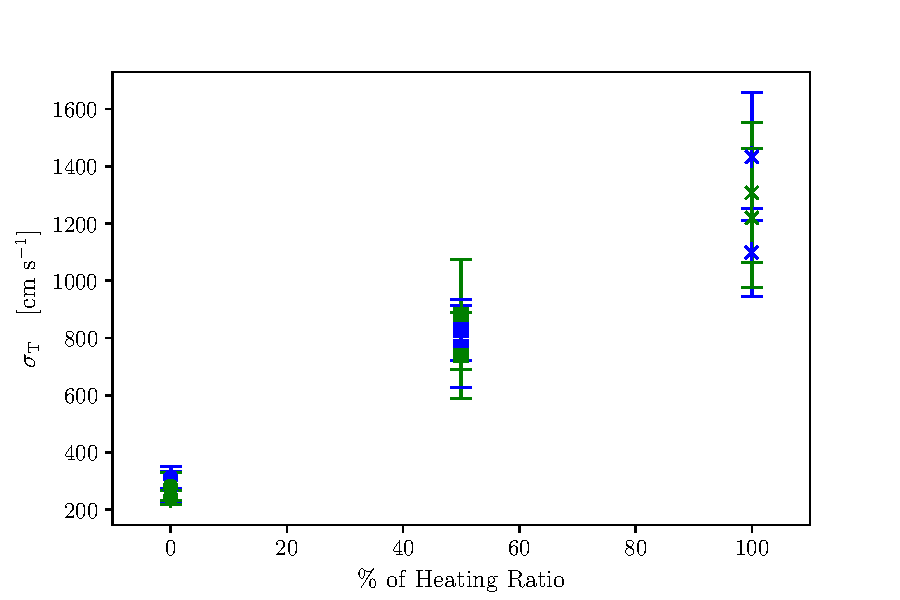
\includegraphics[width=0.5\textwidth]{./img/differentialmach.pdf}\label{fig:diffrms}}
      \hfill
        \subfloat[Dependency of the buoyancy jump on the initial temperature gradient.]{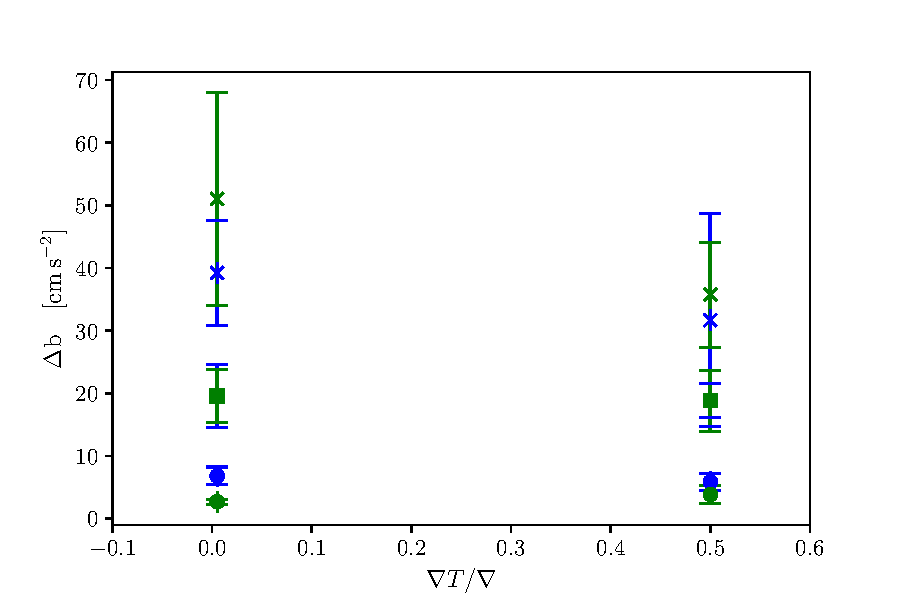
\includegraphics[width=0.5\textwidth]{./img/differentialdelb.pdf}\label{fig:diffjump}}
	\hfill
	\caption{Dependency of the parameters needed to compute the bulk-Richardson number on the initial simulation setup. Blue dots represent the upper boundary, green dots the lower boundary.}
	\label{fig:diffparam}
\end{figure}
As mentioned more than once in the previous chapters, the goal of this work is to perform a \textit{differential} study of the CBM problem. To achieve this, we run four simulations (which provided us 8 boundaries to analyze) varying differentially the stratification and the turbulent regime. 

Following the nomenclature we used in the previous section we hence run the six following simulations: 2d0.5-100 (where $\nabla T / \nabla = 0.5$ and the heating ratio is  $3.6 \times 10^{15} \mathrm{erg/s}$), 2d0.005-100, 2d0.5-050, 2d0.005-050, 2d0.5-005 and 2d0.005-005.

We have no direct control over the turbulent Mach number, but we have it on the heating function. We initialized two different heating ratios, specifically $100 \ \%$ and $5 \ \%$ of the reference value of $3.6 \times 10^{15} \mathrm{erg/s}$. In Figure (\ref{fig:diffrms}) we show the linear dependency of the turbulent Mach number as a function of the heating ratios. This result is a powerful tool to forecast a priori in future simulations the resulting bulk-Richardson numbers.

In order to vary differentially the fluid stratification (hence $\Delta b$), we initialized our simulation setups with three different values for the temperature gradient, namely $\nabla T / \nabla = 0.5, \, 0.50$ and  $0.005$. In Figure (\ref{fig:diffjump}) we plot the buoyancy jumps measured in our simulations over the fraction of the initialized temperature gradients. It seems that the data collected for the most stable stratification ($\nabla T / \nabla = 0.005$) shows a higher value for $\Delta B$ compared to the least stable one, but this definitely does not reflect the change of two orders of magnitude of the initialized values. We believe that this the consequence of two factors. 

The first cause for this discrepancy might be the spikes in the Brunt-Väisälä frequency analyzed in section (\ref{single2d}). It is unclear if the magnitude of these spikes exhibit a non-linear behavior, and a further investigation of such a phenomenon is necessary. 

The second reason is shown in Figure (\ref{fig:diffcorr}). As already mentioned in multiple occasions, the buoyancy jump $\Delta b$ is the thermodynamical term in the bulk-Richardson number that encapsulates the information about the stratification, in contrast to the hamiltonian term $\sigma_{\mathrm{T}}$. We found instead a clear relation between $\Delta b$ and $\sigma_{\mathrm{T}}$. We impute this correlation to the deformations imprinted by stronger turbulent convective blobs to the boundary. This in fact leads to a wider boundary thickness, which is the domain over which we integrate Equation (\ref{eq:buoyancyjump}). The data collected by us on the boundary thickness as a function of the turbulent regime confirms this hypothesis.

The turbulent length scale $L$ also shows an increasing trend with the Mach number.

\begin{figure}[t!]
\centering
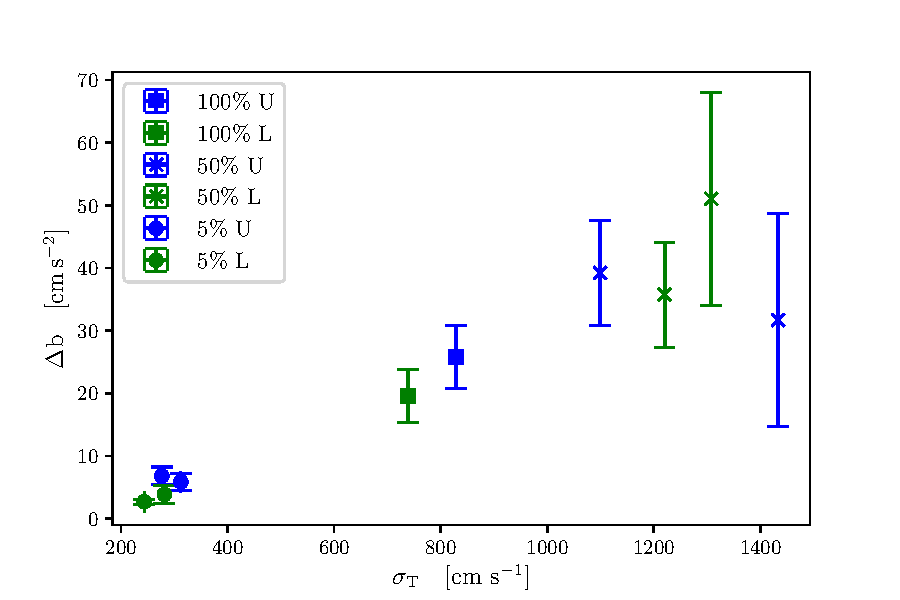
\includegraphics[width=0.7\textwidth]{./img/differentialcorr.pdf}
\caption{Normalized entrainment rate against bulk Richardson number. The error bast are one standard deviation on the mean values.}
\label{fig:diffcorr}
\centering
\end{figure}


Equation (\ref{bulkrichardson}) can be rewritten as

\begin{equation}\label{eq:logaritmicbulk}
	\log{E} = \log{A} - n \log{Ri_{\mathrm{B}}}.
\end{equation}

Recall that on the left-hand side $E=u_{\mathrm{E}}/\sigma_{\mathrm{T}}$ is the boundary migration speed normalized by the turbulent Mach number, which we calculate by mean of the Lagrangian study in our simulations. On the right-hand side we find the bulk-Richardson number, that we can also calculate for every simulation we run. We plot in Figure (\ref{fig:differential}) the experimental value for $\log E$ over $Ri_{\mathrm{B}}$. As usual color blue stands for the upper boundary and green for the lower one. Dots represent the four runs with $5 \%$ of the heating function, crosses the two ones with $100 \%$.

It is clear that the data collected by us definitely does not span a range large enough to perform a proper differential study. This problem is a consequence of two facts. As previously mentioned it is extremely difficult a priori to forecast, given initial parameters, what bulk-Richardson number will result from one given simulation. In addition to this, a higher bulk-Richardson number (hence a stronger boundary or a lower turbulent Mach number) requires more computational resources, which we could not afford by the time we realized the problem. In fact, simulating a stiffer boundary requires a better refinement of the grid. In the case of a lower entrainment rate instead, the system needs to be simulated for a longer time, because the boundary moves at a lower speed.

On the other side, reaching a lower bulk-Richardson number would not be relevant for most applications.

\begin{figure}[t!]
\centering
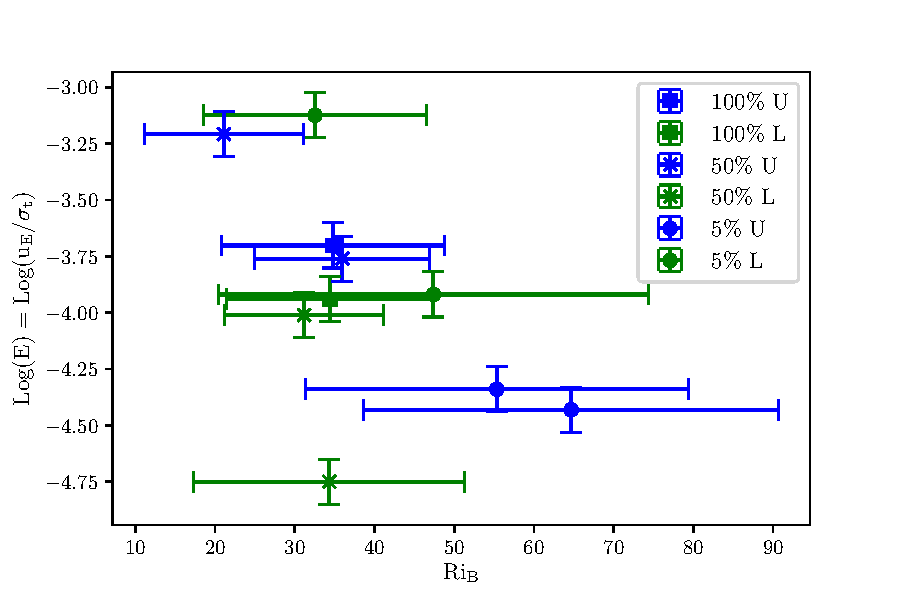
\includegraphics[width=0.7\textwidth]{./img/differential2d.pdf}
\caption{Normalized entrainment rate against bulk Richardson number. The error bars are the standard deviations of the quantities.}
\label{fig:differential}
\centering
\end{figure}

As it can be seen at a first glance, there is no clear correlation between the bulk-Richardson number and the normalized migration velocity over time. It appears that a decreasing trend could be found, which would confirm that the $n$ parameter should assume a negative value. This is what one would expect by a qualitative analysis of the problem. This implies in fact that the stiffer the boundary and the weaker the turbulence regime, the lower the entrained mass. The $A$ parameter instead, which is essential to quantify the mass ingestion, cannot be reliably determined by the data. This is very similar to what was found by \citet{cristini} in their carbon burning shell simulation, when compared their results to the ones of \citet{meakin}. 

We report parametric values of $n=-0.028 \pm 0.007$ and $A=0.071 \pm 0.291$. Both $n$ and $A$ are one order of magnitude lower than the 3D reference values that can be found in the literature. Nevertheless for no reason we would expect that the parameters extracted for a 2D setup would agree with the three-dimensional case.

The error values clearly show that the data range is not wide enough to perform an accurate differential study. Future runs that were not possible during the master project will reach bulk-Richardson numbers of one order of magnitude higher than the ones obtained for this work. This will be achieved primarily by using a non-uniform Cartesian grid which is implemented in SHL. This will help us better refine the convective boundary regions and avoid wasting computational resources to resolve the stable layers above and below.

\section{3D simulations}
\begin{figure}[b!]
      \centering
        \subfloat[Mach number profile over time.]{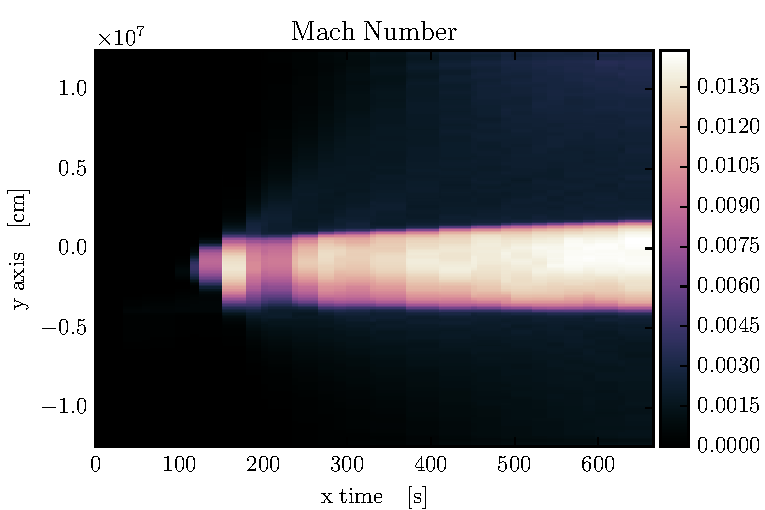
\includegraphics[width=10cm]{./img/3dmachprofile.pdf}\label{fig:3dmachprofile}}
     \centering
	\hfill
        \subfloat[Entrainment of passive scalar from the upper stable region into the convective region.]{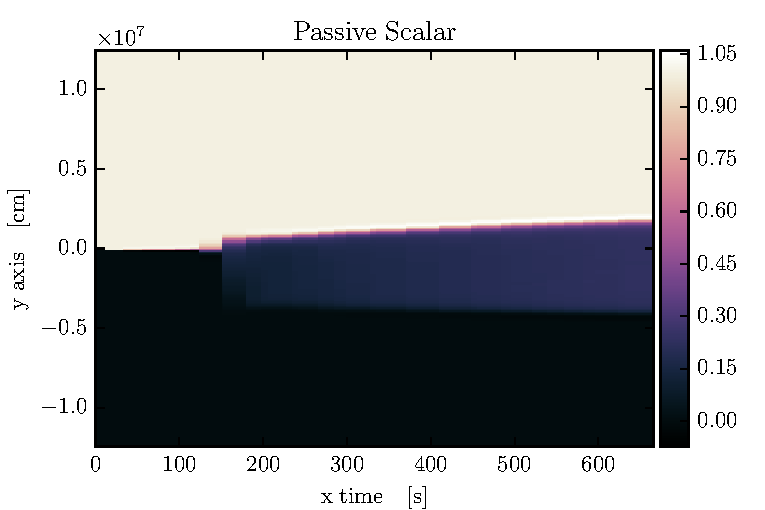
\includegraphics[width=10cm]{./img/3dpassivescalar.pdf}\label{fig:3dpsprofile}}
	\caption{Time evolution of a 3D run for the Mach number and the upper passive scalar. In comparison to the 2D case less output files were saved, hence the lower resolution in time.}
	\label{fig:3dsingle}
\end{figure}
After having correctly tuned the heating function in a 2D setup, we switched to a 3D setup. Only one simulation was run: 3d0.10-100. In fact, because of the problems discussed in the differential study section, we want to make sure that we can successfully outdistance the bulk-Richardson numbers before running other computationally very expensive 3D runs.

The simulation was run on the JUQUEEN machine at Jülich Supercomputing Center (JSC) and scaled over one rack ($16384$ cores) for four days. Although SLH scales very well even on tens of thousands of cores, on JUQUEEN a very high number of CPU hours was needed, primarily because the PowerPC\textregistered \ A2 processors (IBM) of JUQUEEN are optimized to obtain the highest efficiency in terms of computations per watt, rather that per core. 
 
 Only one output every 500 time steps was saved, hence the lower resolution in time for the plots compared to the 2D analysis. This was not necessary to reduce the output size (around $300 \, \mathrm{GB}$ total), but to avoid to spend too many CPU hours in I/O processing.
\subsection{Evolution of a 3D run}

\begin{figure}[t!]
\centering
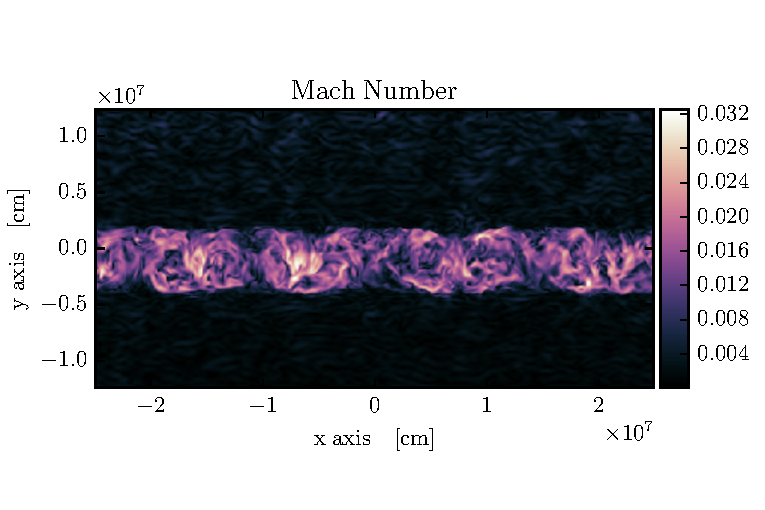
\includegraphics[width=0.6\textwidth]{./img/3dmach.pdf}
\caption{Mach number of a 3D run at about $t=500 \, \mathrm{min}$.}
\label{fig:3dmach}
\end{figure}

The physical setup was mapped on a uniform Cartesian grid with $512 \times 256 \times 512$ cells. In analogy with the 2D setup, we implemented wall boundary conditions for the vertical direction, and periodic boundaries for the horizontal ones. The same usual time-dependent gaussian-shaped heating function was furthermore implemented, with the same heating rate.

Similarly to the 2D case, convection starts at $t \simeq 150 \, \mathrm{min}$, and in Figure (\ref{fig:3dsingle}) the growth of the convective region by entrainment of stable medium is visible.

The 3D case shows also a Mach number of the turbulent flow constant in time over the run, as shown in Figure (\ref{fig:3dmachprofile}), but compared to the 2D Mach number in Figure (\ref{fig:2dmachprofile}) it is significantly lower. This result was expected because, as previously mentioned, three-dimensional turbulence has a different behavior compared to the two-dimensional one. In our cases the 3D turbulence standard deviation was always a factor of a few lower than in the 2D case, which is in agreement with what found by \citet{meakin} in their core-convection simulation. 

The entrainment plotted over time in Figure (\ref{fig:3dpsprofile}) is also roughly linear and qualitatively resembles the 2D result, with the upper and lower boundaries that are migrating upward and downward respectively.
The different turbulence configurations between the 2D and 3D case can be also better understood by comparing Figure (\ref{fig:3dmach}) with Figure (\ref{fig:machhighres}). In Figure (\ref{fig:differentialmach}) we showed that the better the resolution, the more refined and complex the turbulent structure. When considering a 3D output, even by looking at a $512 \times 256$ section of the grid, the Mach number already shows a very complex and convoluted shape, comparable in complexity to the $2048 \times 1024$ 2D case. This obviously has an impact on the entrainment dynamics. Notice that also in this case the Mach number is roughly the half of the 2D case. 


In Figure (\ref{fig:3dpassive}) we plot, as we did for Figure (\ref{fig:2dpassive}), the upper passive scalar density advection. In Figure (\ref{fig:3dpassive2accretion1}) the onset of convection is visible by the presence of the fist convective blobs, that over time fill the convective region as visible in Figure (\ref{fig:3dpsprofile}). Notice that in the 3D case the passive scalar is advected fairly homogeneously in the convective layer, and the problem described in Figure(\ref{fig:topology}) for the boundary detection did not appear. This is another consequence of the previously mentioned 3D turbulent cascade, that helps spread the passive scalar in the convective region better than in the 2D case.

\begin{figure}[t!]
      \centering
      \subfloat[Onset of convective blobs at $t \simeq 150 \, \mathrm{min}$]{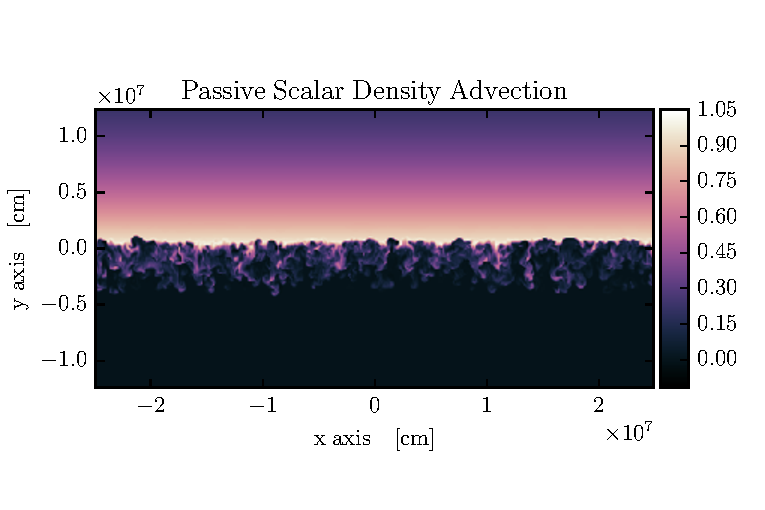
\includegraphics[width=10cm]{./img/3dpassive2accretion1.pdf}\label{fig:3dpassive2accretion1}}
     \centering
	\hfill
	\subfloat[Passive scalar advection at $t \simeq 600  \, \mathrm{min}$.]{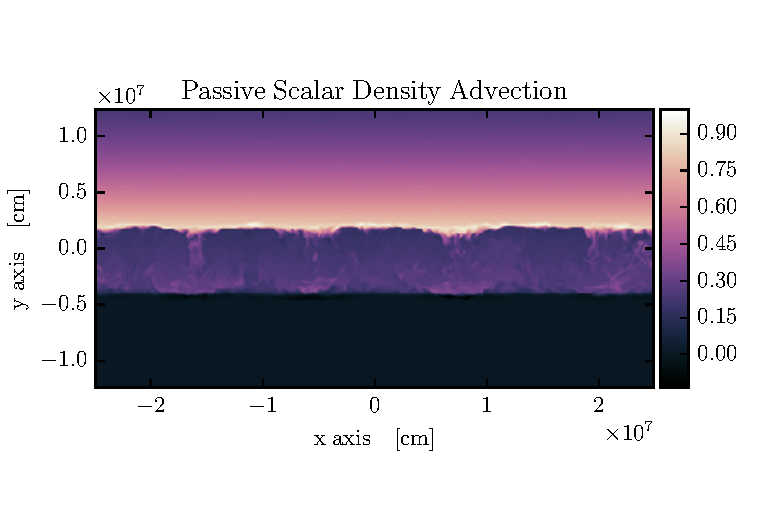
\includegraphics[width=10cm]{./img/3dpassive2accretion2.pdf}\label{fig:3dpassive2accretion2}}
	\caption{Passive scalar density advection for the 3D run. Notice the different shape of the convective blobs compared to Figure (\ref{fig:2dpassive}).}
	\label{fig:3dpassive}
\end{figure}

